%% ----------------------------------------------------------------
%% Thesis.tex -- MAIN FILE (the one that you compile with LaTeX)
%% ---------------------------------------------------------------- 

% Set up the document
\documentclass[a4paper, 12pt, oneside]{Thesis}  % Use the "Thesis" style, based on the ECS Thesis style by Steve Gunn
\graphicspath{{./images/}}  % Location of the graphics files (set up for graphics to be in PDF format)

% Include any extra LaTeX packages required
\usepackage[square, numbers, comma, sort&compress]{natbib}  % Use the "Natbib" style for the references in the Bibliography
\usepackage{verbatim}  % Needed for the "comment" environment to make LaTeX comments
\usepackage{vector}  % Allows "\bvec{}" and "\buvec{}" for "blackboard" style bold vectors in maths
\hypersetup{urlcolor=blue, colorlinks=true}  % Colours hyperlinks in blue, but this can be distracting if there are many links.
\usepackage{graphicx} % This package is for inserting pictures, this package
\usepackage{fancyhdr}
\usepackage[export]{adjustbox}
\usepackage{subcaption} %for the multi pictures in one place
\usepackage{tikz-uml} % for drawing the class diagrams
\usepackage{multirow}
%% ----------------------------------------------------------------
\begin{document}
\frontmatter      % Begin Roman style (i, ii, iii, iv...) page numbering

% Set up the Title Page
\title  {SIMULATION OF A NOVEL MAC PROTOCOL WITH NS3}
\authors  {\texorpdfstring
            {\href{1734634}{Agbeve, Douglas Dziedzorm}}
            {Agbeve, Douglas Dziedzorm}
            }
\addresses  {\groupname\\\deptname\\\univname}  % Do not change this here, instead these must be set in the "Thesis.cls" file, please look through it instead
\date       {\today}
\subject    {}
\keywords   {}

\maketitle
%% ----------------------------------------------------------------

\setstretch{1.3}  % It is better to have smaller font and larger line spacing than the other way round

% Define the page headers using the FancyHdr package and set up for one-sided printing
\fancyhead{}  % Clears all page headers and footers
\rhead{\thepage}  % Sets the right side header to show the page number
\lhead{}  % Clears the left side page header

\pagestyle{fancy}  % Finally, use the "fancy" page style to implement the FancyHdr headers

%% ----------------------------------------------------------------
% Declaration Page required for the Thesis, your institution may give you a different text to place here
\Declaration{

\addtocontents{toc}{\vspace{1em}}  % Add a gap in the Contents, for aesthetics

I, Douglas Dziedzorm Agbeve, declare that this thesis titled, `SIMULATION OF A NOVEL MAC PROTOCOL WITH NS3' and the work presented in it are my own. I confirm that:

\begin{itemize} 
\item[\tiny{$\blacksquare$}] This work was done wholly or mainly while in candidature for a research degree at this University.
 
\item[\tiny{$\blacksquare$}] Where any part of this thesis has previously been submitted for a degree or any other qualification at this University or any other institution, this has been clearly stated.
 
\item[\tiny{$\blacksquare$}] Where I have consulted the published work of others, this is always clearly attributed.
 
\item[\tiny{$\blacksquare$}] Where I have quoted from the work of others, the source is always given. With the exception of such quotations, this thesis is entirely my own work.
 
\item[\tiny{$\blacksquare$}] I have acknowledged all main sources of help.
 
\item[\tiny{$\blacksquare$}] Where the thesis is based on work done by myself jointly with others, I have made clear exactly what was done by others and what I have contributed myself.
\\
\end{itemize}
 
 
Signed:\\
\rule[1em]{25em}{0.5pt}  % This prints a line for the signature
 
Date:\\
\rule[1em]{25em}{0.5pt}  % This prints a line to write the date
}
\clearpage  % Declaration ended, now start a new page

%% ----------------------------------------------------------------
% The "Funny Quote Page"
\pagestyle{empty}  % No headers or footers for the following pages

\null\vfill
% Now comes the "Funny Quote", written in italics
\textit{''\ldots Nothing puzzles God''}

\begin{flushright}
    Chinua Achebe
\end{flushright}

\vfill\vfill\vfill\vfill\vfill\vfill\null
\clearpage  % Funny Quote page ended, start a new page
%% ----------------------------------------------------------------

% The Abstract Page
\addtotoc{Abstract}  % Add the "Abstract" page entry to the Contents
\abstract{
\addtocontents{toc}{\vspace{1em}}  % Add a gap in the Contents, for aesthetics

\ldots

}

\clearpage  % Abstract ended, start a new page
%% ----------------------------------------------------------------

\setstretch{1.3}  % Reset the line-spacing to 1.3 for body text (if it has changed)

% The Acknowledgements page, for thanking everyone
\acknowledgements{
\addtocontents{toc}{\vspace{1em}}  % Add a gap in the Contents, for aesthetics

acknowledgements \ldots

}
\clearpage  % End of the Acknowledgements
%% ----------------------------------------------------------------

\pagestyle{fancy}  %The page style headers have been "empty" all this time, now use the "fancy" headers as defined before to bring them back


%% ----------------------------------------------------------------
\lhead{\emph{Contents}}  % Set the left side page header to "Contents"
\tableofcontents  % Write out the Table of Contents

%% ----------------------------------------------------------------
\lhead{\emph{List of Figures}}  % Set the left side page header to "List if Figures"
\listoffigures  % Write out the List of Figures

%% ----------------------------------------------------------------
\lhead{\emph{List of Tables}}  % Set the left side page header to "List of Tables"
\listoftables  % Write out the List of Tables

%% ----------------------------------------------------------------
\setstretch{1.5}  % Set the line spacing to 1.5, this makes the following tables easier to read
\clearpage  % Start a new page
\lhead{\emph{Abbreviations}}  % Set the left side page header to "Abbreviations"
\listofsymbols{ll}  % Include a list of Abbreviations (a table of two columns)
{
% \textbf{Acronym} & \textbf{W}hat (it) \textbf{S}tands \textbf{F}or \\
\textbf{TDMA} & \textbf{T}ime \textbf{D}ivision \textbf{M}ultiple \textbf{A}ccess \\
\textbf{RFID} & \textbf{R}adio \textbf{F}requency \textbf{I}dentification \\
\textbf{MAC} & \textbf{M}edia \textbf{A}ccess \textbf{C}ontrol
}

%% ----------------------------------------------------------------
%\clearpage  % Start a new page
%\lhead{\emph{Physical Constants}}  % Set the left side page header to "Physical Constants"
%\listofconstants{lrcl}  % Include a list of Physical Constants (a four column table)
{
% Constant Name & Symbol & = & Constant Value (with units) \\
%Speed of Light & $c$ & $=$ & $2.997\ 924\ 58\times10^{8}\ \mbox{ms}^{-\mbox{s}}$ (exact)\\

%}

%% ----------------------------------------------------------------
%\clearpage  %Start a new page
%\lhead{\emph{Symbols}}  % Set the left side page header to "Symbols"
%\listofnomenclature{lll}  % Include a list of Symbols (a three column table)
%{
% symbol & name & unit \\
%$a$ & distance & m \\
%$P$ & power & W (Js$^{-1}$) \\
%& & \\ % Gap to separate the Roman symbols from the Greek
%$\omega$ & angular frequency & rads$^{-1}$ \\
%}
%% ----------------------------------------------------------------
% End of the pre-able, contents and lists of things
% Begin the Dedication page

\setstretch{1.3}  % Return the line spacing back to 1.3

\pagestyle{empty}  % Page style needs to be empty for this page
\dedicatory{for my Nice \ldots}

\addtocontents{toc}{\vspace{2em}}  % Add a gap in the Contents, for aesthetics


%% ----------------------------------------------------------------
\mainmatter	  % Begin normal, numeric (1,2,3...) page numbering
\pagestyle{fancy}  % Return the page headers back to the "fancy" style
\lhead{\emph{\leftmark}}
%\fancyhead[LE]{\nouppercase\leftmark}% LE -> Left part on Even pages
%\fancyhead[RO]{\nouppercase\rightmark}% RO -> Right part on Odd pages
%\fancyfoot[LE,RO]{\thepage}
% Include the chapters of the thesis, as separate files
% Just uncomment the lines as you write the chapters

\chapter{Introduction}

The later part of the past decade has seen a tremendous increase in the research of Internet of Things (IoT) devices mostly geared towards energy efficiency.
This is in part, due to the fact that IoT devices have an underlining positive factor of having to save energy usage and hence must be design as not excessively use energy in itself.
Not only do these interconnected devices provide comfort but have also become critical parts of our daily lives: saving lives, expediting interactions and transactions.
Another factor that fueled the advancement in the research of energy efficient IoT devices is the enormous progress made in the field of Machine learning specifically Reinforcement learning.\\\\
Maximizing a numerical reward signal by learning which actions to take in a given situation is what Reinforcement learning is about.
The actions to take by the learning agent pertaining to various situations are not preprogrammed into the learner, but instead this is discovered by taking the actions that maximize the reward margin\cite{Sutton&Barto}. This works in the cycle of sense-action-goals and learning is from immediate interactions with the environment.\\\\
The APT-MAC protocol, which is the focus of this paper, seeks to solve the problem of the reliance on battery.
The protocol utilizes the Multi-Arm Bandit algorithm, a reinforcement learning algorithm, in tandem with Radio-frequency identification (RFID) signals to enable battery-free communication of wireless devices\cite{Maselli}.\\\\
The aim of this work is to simulate the APT-MAC protocol in NS3 and in comparison to the static TDMA protocol.

\section{The Protocols}
Even though the quality of a network service is a cooperative effort of all the stack of communication protocols, the MAC layer is of a peculiar importance as it handles the sharing of the medium on which all other upper-layered protocols depend.
MAC protocols do not only solve the problem of medium sharing, hence, support for reliable communication but also, in Wireless Sensor Networks, control of energy utilization, achieve through duty cycling and retransmissions or transmission power control\cite{Yigitel&Durmaz&Ersoy}.\\\\
In wireless sensor network, the MAC protocols are broadly classified into contention-based MAC protocols and scheduled-based MAC protocols depending on how he medium is accessed\cite{Pal&Chatterjee}.\\\\
The medium in a contention-base MAC protocol is accessed by all the nodes and, as the name suggests, the nodes contend for access to the medium this may result in collision hence, to prevent collision access to the medium is negotiated through probabilistic coordination.
A sending node listens to shared medium before sending, if the medium is busy, sending is halted for a specified period of time before retrying.
Examples of contention-based MAC protocols used in wireless sensor network are ALOHA (Additive Link On-line Hawaii System)and CSMA (Carrier Sense Multiple Access)\cite{Tanenbaum&Wetherall}.\\\\
Nodes' medium access in a schedule-based MAC protocol is split into either frequency, Frequency Division Multiple Access, or time, that is, Time Division Multiple Access, or orthogonal pseudo - noise codes (Code Division Multiple Access).
Collision is prevent in the medium by making different nodes access the medium in their designated time or frequency and hence not interfering with each other.\\\\
This section deals with the description of the protocol: APT-MAC and Time Division Multiple Access (TDMA).

\subsection{TDMA}
In TDMA, the total duration of communication is divided into fixed number of time slots.
Time slots are configured into time-frames that are repeated periodically.
Each node is allocated a time slot in a time-frame and is allowed to only transmit in that time slot.
The TDMA frame structure has extra overhead; preamble and trail bits, added to the information message or bits.
Time slots are what make up the information bits/message.
Figure \ref{fig:frame_structure} shows the details of the frame structure.\newline
\textbf{Preamble:} contains the address and synchronization information of the base (sink) node and the identification information of the other nodes.\newline
\textbf{Guard time:} necessary to prevent time-drifting over time.\newline
\textbf{Trail bit:} for error detection in the form of checksum or cyclic redundancy check.\newline
\begin{figure}[h]
    \centering
    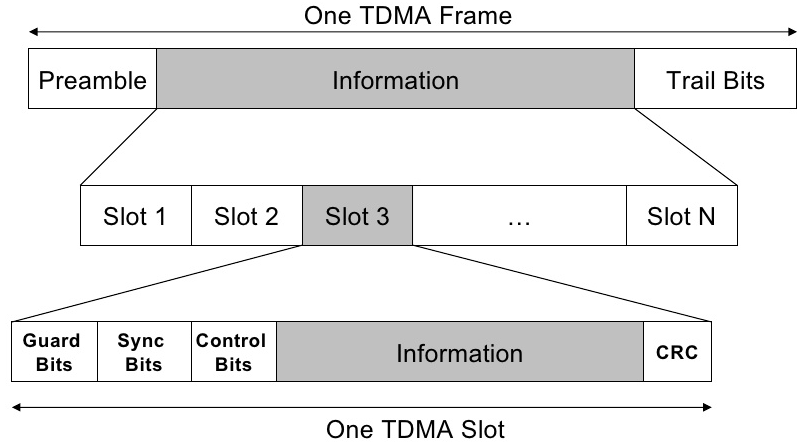
\includegraphics[scale=0.5]{frame_structure}
    \caption{Frame Structure}
    \label{fig:frame_structure}
\end{figure} \newline
The inadequacies of TDMA, chief among them with respect to the aim of the referenced paper \cite{Maselli}, is static slot assignment.
The slots are assigned before transmission and does not change whatsoever during the transmission process, this does not serve the purpose of a protocol that is needed to scale according to the transmission requirements of the nodes.

\subsection{APT-MAC}
APT-MAC protocol is a zero configuration - manual configuration not needed - mac protocol.
Reinforcement learning is utilized to learn the required rate of transmission of each active node and continually update the transmission requirements of nodes.
An overview of the reinforcement learning algorithm is given, followed by how it is used the APT-MAC protocol.
\subsubsection{Multi-Arm Bandit}
    
\subsubsection{APT-MAC protocol overview}
The "battery-freeness" of the protocol is as a result of the use of sensor-augmented RFID tags.

During initialization, the reader sends discovery queries to all nodes and each is assigned a unique identification.
In querying tags in such a way as to minimize the difference between the sensor's data generation time and the time of delivery of data to the reader, the Multi-Arm Bandit, describe above, is used.
The reader, agent in this case, queries each node - set of actions - and can be in one of two states: querying or ready to query.
Expected reward is calculated with the formula \ref{expected_reward} with the expected reward of each action stored in vector $Q$.
\begin{equation}
    Q(a_i)(n+1) = Q(a_i)(n)+\alpha(Reward - Q(a_i)(n))
    \label{expected_reward}
\end{equation}
$n$ is the time slot of the query, $a_i$ is the action of querying tag $i$ and $\alpha$ is the learning rate.\newline
A more detailed explanation of the protocol, such as the learning rate parameter and theevaluation of the $Reward$ can be found in \cite{Maselli}.
 % Introduction

\chapter{Simulation}
The activities of the simulation is described in this chapter.
An overview of NS-3 is given, which is then followed by the actions taken, setup
used, assumptions made and overall explanation of the simulation.

\section{NS-3}
A discrete event network simulator, NS-3 is used extensively in network research
and education. The workings and performance of packet data network are modelled
and NS-3 provides a platform for the simulation and experimentation of various
packet-based research. C++ and Python are the predominant language in which NS-3
is written with \textit{waf} as the build system. Design of NS-3 capitalizes on
the object oriented nature of these languages\cite{nsonline}.\\\\
There are various components of packet-based network, fundamentally there are the
endpoint devices, routers,NIC devices ,switches and the medium of exchange.
These components,however in NS-3, are abstracted to reflect what the components
actually do. The endpoint devices are called \textit{Nodes}, exchange medium
- \textit{Channel} and the applications that are generating the packets are 
\textit{Applications} just to name a few. The file/folder structure of a simulation
consist of a model which depicts the fine details of the simulation, a helper that
is supposed to include files containing the installation helper functions, an 
example folder to implement an example of the simulation. There are also doc and 
tests folders and the just as their names suggest they hold documentation and tests
files.\\\\
Installation of the NS-3 is not needed to get a simulation running, as the examples 
or experiments can be run using the binary files gotten from the build process.
It is actually not recommended to do installation of NS-3. Installation in this case
refers to running the command \textbf{\textit{./waf install}}.

\section{Setup}
The simulation was performed on a Gentoo Linux flavor computer with a 64 bit Intel
Eight-Core processor with model name \textit{Intel(R) Core(TM) i7-8565U CPU @
1.80GHz} and RAM of 32GB. Version 3-30 of NS-3 provided the platform on which to
undertake the research. At the time of setting up, this version was the latest most
stable release.\\\\
NS-3 is a voluminous software, the faster processor is needed, as a change to any
file would mean rebuilding the file and its dependencies and those that depend on it.
The version is also critical. Most versions are not backward compatible hence what
works on 3.29 might not work on 3.30 without a little tinkering.\\\\
Gentoo Linux, even though time consuming and quite advance in installation and
setting up, turns to be one of the fastest linux operating systems available. This is
partly due to the fact that source codes are compiled on the host computer with 
specific flags set for optimality.

\section{Components}
For a data packet to move from one endpoint to another, there are components such as,
the packet generating and receiving nodes which will have NIC, the medium(s) through
which the packet traverses also forms a part of the components.\\\\
There are three critical parts, worth mentioning for this simulation; the header which
is attached to the packet, tag-augmented sensor devices and the reader, which, in this
case, is augmented with a server.\\\\
A discussion of the various components follow next.
\subsection{Packet Header}
Various parts of a packet header which is added to a payload enable the packet to get
to its intended destination. A 4-byte(32 bits) header was created, having two fields
of 16 bits each representing the packet type being sent: data packet or broadcast 
and the state of the tag augmented sensor: whether a new data is available for 
transmission or not.\\
\begin{figure}[h!]
\begin{tikzpicture}
    \tikzumlset{font=\tiny\ttfamily}
    \umlemptyclass[x=0,y=0]{Header}{
}{}
\umlclass[x=5.5,y=-2]{AptMacHeader}{
  -m\_id : uint16\_t \\ -m\_type : uint16\_t \\ -m\_stateChange : uint16\_t
}{
  +AptMacHeader() \\ +SetId(id : uint16\_t) : void \\ +GetId (void) : const
  uint16\_t\\ +SetPacketType(ptype : uint16\_t) : void \\ +GetPacketType(void) :
  const uint16\_t \\ +SetStateChange(stateChange : uint16\_t) : void \\ 
  +GetStateChange(void) : const uint16\_t \\ \umlstatic{+GetTypeId(void) : TypeId}\\
  \umlvirt{+Serialize(start : Buffer::Iterator) : const void} \\
  \umlvirt{+Deserialize(start : Buffer::Iterator) : uint32\_t} \\
  \umlvirt{+GetSerializedSize(void) : const uint32\_t} \\
  \umlvirt{+GetInstanceTypeId (void) : const TypeId} \\
  \umlvirt{+Print(\&os : std::ostream) : const void}\\
}
\umlenum[x=11.5,y=-4]{HeaderContents}{
    BROADCAST : uint16\_t \\ DATA : uint16\_t \\ STATECHANGE : uint16\_t
}

%\umlassoc[geometry=-|-, arg1=tata, mult1=*, pos1=0.3, arg2=toto, mult2=1, pos2=2.9, align2=left]{C}{Header}
%\umlunicompo[geometry=-|, arg=titi, mult=*, pos=1.7, stereo=vector]{D}{C}
%\umlimport[geometry=|-, anchors=90 and 50, name=import]{sp2}{sp1}
\umlaggreg[geometry=-|]{AptMacHeader}{HeaderContents}
\umlinherit[geometry=-|]{AptMacHeader}{Header}
%\umlnote[x=2.5,y=-6, width=3cm]{B}{Je suis une note qui concerne la classe B}
%\umlnote[x=7.5,y=-2]{import-2}{Je suis une note qui concerne la relation d'import}
\end{tikzpicture}
\caption{Class Diagram - APT-MAC Header}
\label{fig:headerUML}
\end{figure}\\
The UML class diagram is illustrated in Figure \ref{fig:headerUML}. The \emph{
constructor, getter and setter} functions are for their usual purposes. \emph{
Serialize} function puts the various fields of the header in series by writing them
from host-order to network-order and the \emph{Deserialize} reads from network-order
to host-order. \emph{Enum HeaderContents} holds the value of the various fields of
the header.

\subsection{Tag Augmented Sensor Devices}
Devices in a smart home are broadly classified under three categories: periodic
(e.g., temperature sensors), real-time (e.g., joystick, cameras) and event based 
(e.g., presence detector, remote of appliances)\cite{Maselli}. The state changes
of the various devices were modelled according to Markov Chains\cite{Tolver}.\\
\begin{centering}
\begin{figure}[h!]
    \begin{subfigure}[b]{.5\textwidth}
        \centering
        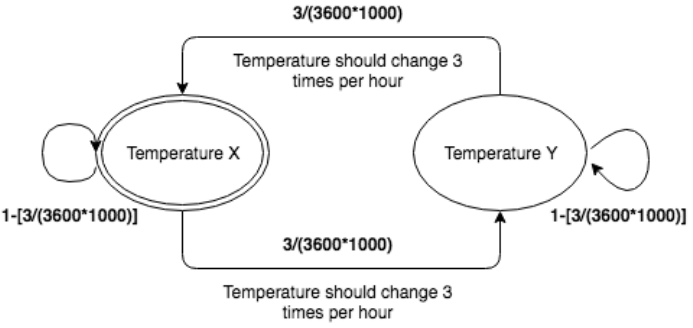
\includegraphics[width=1\linewidth]{temperature-sensor}
        \caption{Temperature Sensor model}
        \label{fig:temperature-sensor}
    \end{subfigure}
    \begin{subfigure}[b]{.5\textwidth}
        \centering
        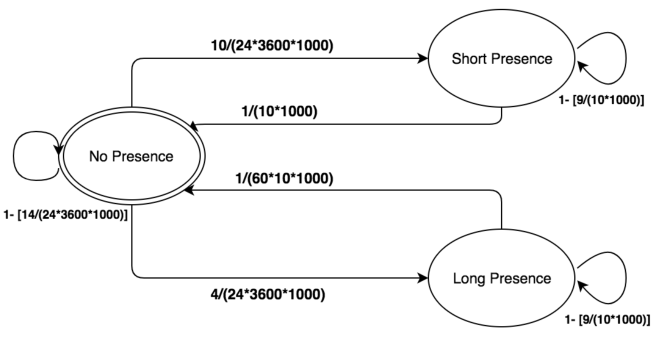
\includegraphics[width=1\linewidth]{presence-sensor}
        \caption{Presence Sensor model}
        \label{fig:presence-sensor}
    \end{subfigure}
    \begin{subfigure}[b]{.5\textwidth}
        \centering
        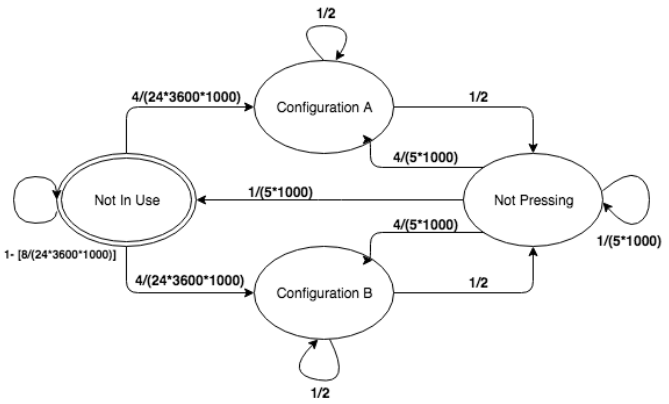
\includegraphics[width=1\linewidth]{tv-remote}
        \caption{TV Remote model}
        \label{fig:tv-remote}
    \end{subfigure}
    \begin{subfigure}[b]{.5\textwidth}
        \centering
        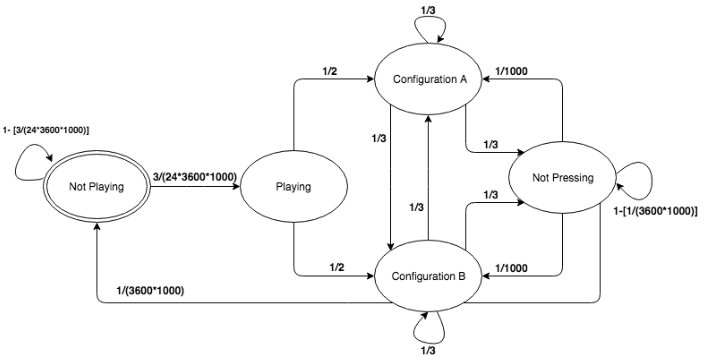
\includegraphics[width=1\linewidth]{joysick-sensor}
        \caption{Joystick model}
        \label{fig:joysick-sensor}
    \end{subfigure}
\end{figure}
\end{centering}\\
Figures \ref{fig:temperature-sensor} to \ref{fig:joysick-sensor}, taken from
\cite{Maselli}, depicts the transition probabilities of the various states a device
could be in. The state change is based on time. Taking fig \ref{fig:temperature-sensor}
for instance, it was found that a temperature sensor produces new data three times in
an hour hence the various probabilities with respect to time in milliseconds.
There are two states in with a temperature sensor and with a probability of 
$3/(3600*1000)$ it changes from, lets say, state X to Y or vice versa and with
$1-3/(3600*1000)$ stays in its state.\\\\
\begin{centering}
\begin{figure}[h!]
    \begin{tikzpicture}
        \tikzumlset{font=\tiny\ttfamily}
        \umlemptyclass[x=-3.5,y=0]{Application}{
        }{}
        \umlclass[x=2.5,y=-2]{SensorNode}{
            -m\_port : uint16\_t \\ -m\_PreState : uint16\_t \\ m\_received :
            uint64\_t \\ -m\_socket : Ptr$\langle$Socket$\rangle$ \\
            -m\_lossCounter : PacketLossCounter
        }{
        +SensorNode() \\
        \umlvirt{$\sim$SensorNode} \\
        \umlvirt{-StartApplication(void) : void} \\
        \umlvirt{-StopApplication(void) : void} \\
        \umlvirt{\#DoDispose(void) : void} \\
        -HandleRead(socket : Ptr{\tiny$\langle$}Socket{\tiny$\rangle$})
        : void \\ -indexOfLargestProb({\tiny\&}matrix : Matrix) : int \\
        -CopyMatrix({\tiny\&}from : Matrix, {\tiny\&}to : Matrix) : void \\
        -MultMatrix({\tiny\&}trsMtx : const Matrix, {\tiny\&}trsMtxb
        : const Matrix) : Matrix \\
        \umlstatic{+GetTypeId(void) : TypeId} \\ +GetLost(void) : const uint32\_t \\
        +GetReceived(void) : uint64\_t
    }
    \umltypedef[x=-1.5,y=-6]{Matrix}{}{}
    \umlemptyclass[x=-3.5,y=-3.5,template={T,U}]{std::vector}{}{
    }
    \umlclass[x=4.0,y=-7.5]{SensorNodeHelper}{
        -m\_factory : ObjectFactory \\
        -m\_server : Ptr{\tiny$\langle$}SensorNode{\tiny$\rangle$}
    }
    {
        +SensorNodeHelper() \\ +SensorNodeHelper(port : uint16\_t) \\
        +SetAttribute(name : std::string , {\tiny\&}value : const AttributeValue) \\
        +Install(c : NodeContainer) : ApplicationContainer \\
        +GetServer(void) : Ptr{\tiny$\langle$}SensorNode{\tiny$\rangle$}
    }
    \umlenum[x=9.5,y=-4.1]{HeaderValidation}
    {
        BROADCAST : uint16\_t \\ BROADCAST\_REPLY : uint16\_t \\ DATA : uint16\_t
        \\ DATA\_REPLY : uint16\_t \\ STATE\_CHANGED : uint16\_t \\
        STATE\_NOT\_CHANGED : uint16\_t
    }{}
    \umldep[geometry=-|]{Matrix}{std::vector}
    \umldep[geometry=-|]{SensorNode}{Matrix}
    \umlinherit[geometry=-|]{SensorNode}{Application}
    \umlaggreg[geometry=-|]{SensorNode}{HeaderValidation}
    \end{tikzpicture}
    \caption{Class Diagram - Sensor Nodes}
    \label{fig:SensorNodes}
\end{figure}
\end{centering}
Markov Chain with a transition probability, say \textbf{$T$}, and an initial state
probability vector distribution \textbf{$q$}. The probability of the chain being in
state $S_i$ after $n$ steps is the $i^{th}$ entry in the vector given by
\begin{equation}
    q^n = q*( T)^n
    \label{eq:markov}
\end{equation}
To simulate the state change based on equation \ref{eq:markov} and also, taking into
account the discrete time with which the changes occur. The next state vector
probability was computed with the $n^{th}$ step being the current time stamp of the
simulation.\\\\
For each tag-augmented sensor node, when a packet is received, the header is checked
to determine the type of packet. If the packet is that of broadcast, a broadcast
reply is automatically sent to the reader with a payload of the current data.
A data request packet require the sensor node to reply with data. A current state
vector probability is calculated and the index with the maximum value is the state 
of the sensor node. If the computed current state is the same as the previous state,
a \textit{state-not-changed} flag is set in the packet header, data reply flag is 
also set and packet sent to the reader.\\\\
The difference in the various sensors is their transition matrix and the initial
state vector, as shown in \ref{fig:temperature-sensor} - \ref{fig:joysick-sensor},
hence the one class for all the sensor nodes.\\\\
Class diagrams of the \textit{SensorNode} class and its \textit{helper} class are
shown in figure \ref{fig:SensorNodes}. A brief explanation regarding the tasks of
the essential functions of the classes follows.
\begin{itemize}
\renewcommand{\labelitemi}{}
\item \textbf{StartApplication:} the first function run to start the application.
    It sets up a socket, binds it to a local address and configures the function
    to handle a received packet.
\item \textbf{StopApplication:} stops the application by resetting the
    packet-received call back function and closing the socket.
\item \textbf{HandleRead:} this is the packet-received call back function. It is
    invoked when a new packet arrives in the socket or when there is data/packet
    to be read in the socket file. The type of packet received is determined by
    examining the header. A broadcast-reply is sent back to the reader if a broadcast
    packet is received by setting the broadcast-reply flag in the header. For a
    data-request packet, the current state of the sensor node is retrieved from the
    \textit{NextState} function and compared with the previous state. If the states
    (previous and current) are equal, data-reply and state-not-changed flags are set
    in the packet header and if the states differ, state-changed and data-reply
    flags are set. The packet is then sent to the reader.
\item \textbf{NextState:} the state of the sensor node is computed by this function
    which takes the current time stamp as a parameter. \textit{Next-State} is found
    by multiplying previous state vector probability with the time-stamp square of
    the transition probability matrix gotten from multiplying the transition matrix
    time-stamp times, hence the need for a matrix multiplication and copy functions.
\end{itemize}
\textit{SensorNodeHelper} class has functions that aid in the installation of sensors
onto nodes; \textit{Install} function, setting the attributes that were declared in
\textit{GetTypeId} function of the \textit{SensorNode} class with \textit{SetAttribute}
which takes the name of the attributes and the value to be set as parameters. There
are, of course, the constructors and a function that return a pointer to the
associated server.

\subsection{Device Sims}
Rate at which data is generated when device is in use, the quantum of data produced
during usage and the number of times the devices are actually used in a day are but a
few differences between an event-based, periodic, and real-time sensor devices.\\\\
Temperature sensor, Presence sensor, TV remote, Joystick and camera are modelled
to depict their change of state with regard to when packets/data are generated by
these devices over a day-use period. The devices model of the simulation is based
on the usage findings from \cite{Maselli}.
\begin{enumerate}
    \renewcommand{\labelenumi}{\alph{enumi}{.}}
\item \textit{Temperature Sensor:} Only two states which is expected to occur three
    times in an hour, which translates to seventy two $72$ times in a day.\\
    In a simulation time period of a day, \textit{Temperature Sensor} was scheduled
    to append a packet to the packet vector $72$ times. Only one packet is appended
    on each state change. This is done by calling a \textit{GeneratePacket} function.
\item \textit{Presence Sensor:} There are three states; \textit{No Presence,
    Short Presence and Long Presence}. In a daily use, state changes from
    \textit{No Presence} to \textit{Short Presence} 10 times and lasts for 10 seconds
    in the \textit{Short Presence} state and from \textit{No Presence} to
    \textit{Long Presence} 4 times, for 10 minutes that state.\\
    After replying to a query for identification by the \textit{reader}. It schedules
    a \textit{GeneratePacketShort} and \textit{GeneratePacketLong} functions to be
    called 10 and 4 times respectively during the simulation period of a day \textit{
    $(86400s)$}. The functions fill up a packet vector during each call for a period
    of \textit{$10s$} and \textit{$10min$} respectively.
\item \textit{TV remote:} Multiple buttons could put a \textit{TV remote} in an
    \textit{In Use} state from a \textit{Not In Use} state. The different button
    states are two - \textit{Configuration A} and \textit{Configuration B}. There is
    an equal chance of moving from \textit{Not In Use} state to either\textit{
    configurations} and when in any of the \textit{Configurations} there is an equal
    probability of moving to a \textit{Not Pressing} state or staying in the same
    state but no chance of going to another \textit{Configuration} without first having
    to go through a \textit{Not Pressing} state. Having same chance of moving to any
    of other states from the \textit{Not Pressing} state. It is used 10 times a day and
    lasts for approximately \textit{$8s$} per use.\\
    The \textit{TV remote} class is programmed to fill up the packet vector 10 times
    in a day of simulation. The generation of the packets lasts for \textit{$8s$}. During
    this time which the \textit{GeneratePacket} function is called, the various states
    changes are simulated using Markov. When a \textit{Not Pressing} state is returned,
    no packet is added to the vector but for the other two states, packets are added to
    the vector.
\item \textit{Joystick:} With a three times a day usage and an hour long on each use,
    the \textit{Joystick} was simulated to have five states - \textit{Not Playing},
    \textit{Playing}, \textit{Configuration A}, \textit{Configuration B},\textit{
    Not Pressing}. There is equal probability of moving from \textit{Not Playing} state
    to either \textit{Configuration} states and from \textit{Configuration A} or
    \textit{B}
    the \textit{Joystick} moves into a \textit{Not Pressing} state, to a different
    \textit{Configuration} or stays in it's state, all with equal probability and vice
    versa from a \textit{Not Pressing} state.\\
    The generation is packet was scheduled to occur three times and to last for an hour
    on each call, in a daily simulation, thus changing from \textit{Not Playing} to
    \textit{Playing} states. In a \textit{Playing} state, a transition is made through
    all the possible states with equal probabilities. When either \textit{Configuration A}
    or \textit{Configuration B} is returned, a packet is added to the packet vector and
    no packet is appended to the vector in the case of \textit{Not Pressing} returned.
\item \textit{Camera:} Takes a shot of an image size of \textit{$25$KB} which takes
    approximately \textit{$30$s} to send to the querier.\\
    The \textit{GeneratePacket} function is called as soon as the packet vector is empty,
    implying the sending of the \textit{$25$KB} data. The packet generation is scheduled
    at a minute after sending to prevent the camera from seizing the medium.
\end{enumerate}
When a \textit{data request} query is received, the content of the packet vector is checked
for emptiness, if empty, the \textit{STATE\_NOT\_CHANGED} flag is set and reply sent to
the header. The \textit{STATE\_CHANGED} flag is set, added to each packet in the vector
before sending all the packets in the vector, for when the vector is not empty.
The memory tag size of each device is set to $256$\textit{bits} ($32$\textit{bytes}).
\subsection{Querier}
An RFID reader or interrogator, and in this case, a querier is a bridge between an RFID
tag and a controller which, among other things could, read and write data to the tag,
power the tag and relay data to and from the controller\cite{HuntPuglia&Puglia}.\\
Controllers are mainly the part of the system that does the processing of the data on
the tags.\\\\
Querying of tags is done in a slotted time. In each time slot, a request-for-data
packet is sent to the tags with a response of positive or negative data. With TDMA,
discussed earlier, slot assignment is static, not responsive to the demand of the
volume of data available on tag-augmented sensors hence does not scale in this case.
A more scalable and responsive algorithm is proposed in \cite{Maselli}, where for each
time slot a query is made and based on the outcome of the response to the query, more
queries are made to the same tag or not. For a positive response, a reward parameter
is increased and the highest reward value in the reward vector is queried next.
Intuitively, a positive response implies query same tag again.\\
\begin{centering}
    \begin{figure}[h!]
        \begin{tikzpicture}
            \tikzumlset{font=\tiny\ttfamily}
            \umlemptyclass[x=-4.0,y=1]{Application}
            {}{}
            \umlclass[x=3.0,y=-3.5]{Querier}
            {
                -m\_sendEvent : ns3::EventId \\ -m\_bonus : double \\
                -m\_malus : double \\ -m\_learningRate : double \\
                -m\_nodeAddress : std::vector$\langle${ns3::Address}$\rangle$ \\
                -m\_reward : std::vector$\langle${double}$\rangle$ \\
                -m\_sReward : std::vector$\langle${double}$\rangle$ \\
                -m\_peerPort : uint16\_t \\ -m\_peerAddress : ns3::Address \\
                -m\_socket : Ptr$\langle${Socket}$\rangle$ \\ -m\_sent : uint32\_t
            }
            {
                +Querier() \\
                \umlvirt{$\sim$Querier()} \\
                \umlstatic{+GetTypeId(void) : ns3::TypeId} \\
                +SetRemote(ip : ns3::Address , port : uint16\_t) : void \\
                +SetRemote(ip : ns3::Address) : void \\
                \umlvirt{\#DoDispose(void) : void} \\
                \umlvirt{-StartApplication(void) : void} \\
                \umlvirt{-StopApplication(void) : void} \\
                -Send(void) : void \\
                -HandleRead(socket : Ptr$\langle${ns3::Socket}$\rangle$) : void \\
                -UpdateReward(reward : std::vector$\langle${double}$\rangle$ ,
                bonusORmalus : double , index : int) :
                std::vector$\langle${double}$\rangle$ \\
                -SoftMax(reward : std::vector$\langle${double}$\rangle$)
            }
            \umlenum[x=10,y=-9.3]{HeaderValidation}
            {
                BROADCAST : uint16\_t \\ BROADCAST\_REPLY : uint16\_t \\
                DATA : uint16\_t \\ DATA\_REPLY : uint16\_t \\
                STATE\_CHANGED : uint16\_t \\ STATE\_NOT\_CHANGED : uint16\_t
            }
            {}
            \umlclass[x=1,y=-9.0]{QuerierHelper}
            {
                -m\_factory : ObjectFactory
            }
            {
                +QuerierHelper() \\
                +QuerierHelper(ip : Address) \\
                +QuerierHelper(ip : Address , port : uint16\_t) \\
                +SetAttribute(name : std::string, ${\&}$value : AttributeValue
                                const) \\
                +Install(c : NodeContainer) : ApplicationContainer
            }
            \umlinherit[geometry=-|]{Querier}{Application}
            \umlaggreg[geometry=-|]{Querier}{HeaderValidation}

        \end{tikzpicture}
        \caption{Class Diagram - Querier}
        \label{fig:Querier}
    \end{figure}
\end{centering}
\\
The class diagram illustrating the \textit{Querier} class and its helper class are
shown in \ref{fig:Querier}.\\
A discussion of the various function of each class follows next.
\begin{itemize}
    \renewcommand{\labelitemi}{}
\item \textbf{StartApplication:} the function to run in initializing the application.
    Socket is created if there are no existing ones bound to the device and connected
    to a peer address, which, in this case, is a broadcast address. Broadcast is
    enabled on the socket, a packet-received-callback function is set up and 
    finally the \textit{send} function is scheduled to immediately be invoked.
\item \textbf{StopApplication:} called during the cancellation of the simulation.
    Socket is closed and stripped down, the scheduled event is canceled.
\item \textbf{Send:} the Querier broadcast to all the tags to get an inventory of
    tags available. This function takes care of that. Packet is created, the broadcast
    flag in the header is set and sent to the broadcast address.
\item \textbf{HandleRead:} this is the packet-received-callback function, takes a
    socket as parameter and invoked when there are packets to be read from the socket
    file. The header of the packet is checked to determine the type of packet received.
    If a \textit{broadcast\_reply} is received and it is not in the \textit{Querier}
    inventory, it is added to the inventory. A packet with \textit{data-request} flag
    is set and sent back to the tag from which the \textit{broadcast\_reply} is 
    received.\\\\
    For a \textit{data\_reply} packet type, the reward value of the sending tag is
    retrieved and the \textit{state\_changed} flag is checked to determine if a new
    data was sent or not. If a new data was sent, the reward vector is updated with a
    \textit{m\_bonus} value and with a \textit{m\_malus} value if no new data is
    received. \textit{SoftMax} is applied to the reward vector, the index with the
    highest value is gotten which is the same index of the node vector, the 
    \textit{data-request} flag is set and the packet sent to the node with the
    maximum reward value. This cycle continues till the end of the simulation.
\item \textbf{UpdateReward:} updates the reward vector. It takes as parameters the
    reward vector, \textit{bonusORmalus} and the index of node whose reward needs
    updating. A check is made to determine whether the updating is that of 
    \textit{m\_bonus} or \textit{m\_malus} and the reward is updated based on
    \ref{expected_reward}. The function returns the reward vector.
\end{itemize}
The constructor and destructor functions are included. There two versions of
\textit{SetRemote}, one takes only \textit{Address} as parameter and the other
\textit{Address} and \textit{port}, they perform the same function of setting up the
remote address. \textit{GetTypeId} returns the \textit{TypeId} of the class.\\\\

Helper class of \textit{Querier} has similar functions of the \textit{SensorNodeHelper}
in \ref{fig:SensorNodes} and they perform virtually the same duties. As a result,
a further discussion is omitted here.

\subsection{TDMA Reader}
This reader class is implemented in a TDMA fashion. Each query, which is slotted in a
specific time interval, is done sequential and in an endless loop.
\begin{centering}
    \begin{figure}[h!]
        \begin{tikzpicture}
            \tikzumlset{font=\tiny\ttfamily}
            \umlemptyclass[x=-4.0,y=1]{Application}
            {}{}
            \umlclass[x=3.0,y=-3.5]{TDMAQuerier}
            {
                -m\_AddressVector : std::vector$\langle${ns3::Address}$\rangle$ \\
                -m\_peerPort : uint16\_t \\ -m\_peerAddress : ns3::Address \\
                -m\_socket : ns3::Ptr$\langle${ns3::Socket}$\rangle$
            }
            {
                +TDMAQuerier() \\ \umlvirt{$\sim$TDMAQuerier()} \\
                \umlstatic{+GetTypeId(void) : ns3::TypeId} \\
                +SetRemote(ip : ns3::Address , port : uint16\_t) \\
                +SetRemote(ip : ns3::Address) : void \\
                +ScheduleNextTx(socket : ns3::Ptr$\langle${ns3::Socket}$\rangle$)
                : void \\
                \umlvirt{\#DoDispose(void) : void} \\
                \umlvirt{-StartApplication(void) : void} \\
                \umlvirt{-StopApplication(void) : void} \\
                -SendQuery(socket : ns3::Ptr$\langle${ns3::Socket}$\rangle$
                , form : ns3::Address , packet :
                ns3::Ptr$\langle${ns3::Packet}$\rangle$) \\
                -HandleReceive(socket : ns3::Ptr$\langle${ns3::Socket}$\rangle$)\\
                -Send(void) : void


            }
            \umlclass[x=1,y=-9.0]{QuerierHelper}
            {
                -m\_factory : ObjectFactory
            }
            {
                +TDMAQuerierHelper() \\
                +IDMAQuerierHelper(ip : Address) \\
                +TDMAQuerierHelper(ip : Address , port : uint16\_t) \\
                +SetAttribute(name : std::string, ${\&}$value : AttributeValue
                const) \\
                +Install(c : NodeContainer) : ApplicationContainer

            }
            \umlinherit[geometry=-|]{TDMAQuerier}{Application}

        \end{tikzpicture}
    \end{figure}
\end{centering}\\
\textit{StartApplication} function is called at the initiation state of the
\textit{TDMAQuerier} class. It sets up an IPv4 UDP socket, connects to the broadcast,
configures the \textit{SetRecvCallback} function of the \textit{socket} class to
\textit{HandleReceive} which reads packet in the socket file, the \textit{Send}
function queries for device identification is called next and the finally the 
\textit{ScheduleNextTx} is scheduled to be called a minute after initiation, at which
point all devices should be identified.\\\\
The packet type is checked in the \textit{HandleReceive} function, when it is a reply
to broadcast identification and the device is not already in \textit{m\_AddressVector},
it is added. \textit{ScheduleNextTx} function takes socket pointer as an argument,
creates a one-byte packet and schedules \textit{SendQuery} for each device address
in the \textit{m\_AddressVector} vector to be called at $10$\textit{milliseconds}
apart, it starts again when it gets to the final address in the vector.
$10$\textit{milliseconds} was found to be the least inter-slot time capable of
allowing for the devices to be able to log the parameters of interest. The 
\textit{SendQuery} function takes socket pointer, address and packet pointer as
arguments, it adds \textit{DATA\_REQUEST} flag to the header of the packet and sends
it off to the designated address.\\\\
The \textit{Install} function of the \textit{QuerierHelper} class 'installs' the
application on the node. \textit{SetAttribute} sets the various attributes on the
\textit{m\_factory}.

\subsection{Example}
The simulation is set up here. A number of nodes is created depending on the number of
tag-augmented sensors that is of interest. A net-device is installed on each node with
a simple wireless channel/media also installed of $640$\textit{kbps} data rate.
The data rate of the net-device is set at $640$\textit{kbps} \cite{epcglobal}.\\\\
Internet stack is added to the nodes and ipv4 is assigned to each network interfaces.
One of the nodes is selected and on it is installed the \textit{Querier}, it becomes
the reader. The other nodes are the tag-augmented sensors and on each is installed
\textit{SensorNode} which is configured depending on whether it be an event based
sensor, a real-time sensor or a periodic sensor. The start and stop time of the
simulation is indicted and started.
 % Background Theory 

\chapter{Results}
Discussion of the results takes place in this chapter. The chapter begins with
with a description of the data collection process, followed by the parameters
considered for performance analysis and ends with discussion of the results obtained.

\section{Data Collection}
With \textit{CreateDatafile} function of each device class, which is called in the
\textit{Install} function of the helper classes, log files are created to contain
data loss and packet delay values of each device simulated. Packet delay and data
loss are the parameters of interest to evaluate the performance of APT-MAC.
\begin{enumerate}
    \renewcommand{\labelenumi}{}
\item \textit{Packet Delay:} the difference in time between generating a packet data
    and sending to the reader.\\
    A call to \textit{SetPacketGeneratingTime} function at the end of
    \textit{GeneratePacket} function sets the time of packet generation and when a
    packet is sent to the reader, \textit{SetPacketSentTime} is called to set the
    sending time. The difference is thus the packet delay which is log in the packet
    delay log file.
\item \textit{Data Loss:} this is the produced data that is not delivered to the
    reader. Calculated by dividing the amount of data sent by the quantum of data
    produced, the percentage of the result subtracted from $1$ is the data loss.
    Thus it is a percentage.\\
    A counter, \textit{m\_newDataCountProduced}, is kept which is increased,
    a call to \textit{UpdateNewDataProduced()}, anytime a new data is
    produced. The variable, \textit{m\_newDataCountSent}, is increased by a call to
    \textit{UpdateNewDataSent}(), whenever a data packet is sent across to
    the reader. When \textit{m\_queryCounter}, holds the number of
    times a query is received from the reader by a device and increased with a call
    to \textit{UpdateQueryCounter()}, gets to $5$, \textit{data loss} is computed
    as indicated earlier and the value log in the data loss log file. The data loss
    is calculated after every $5$ \textit{data-query} request received by the
    tag-augmented sensor device.
\end{enumerate}
\begin{table}[h!]
    \caption{WORKLOAD SCENARIOS DESCRIPTION}
    \label{tab:WSD}
    \centering
    \begin{tabular} { | c | c | c | c | c | }
        \hline
        \multicolumn{1}{| c }{No. of Sensors}  & \multicolumn{1}{c }{Scenario}
                                             & \multicolumn{1}{ c }{Joystick}
                                             & \multicolumn{1}{ c }{Remote}
                                             & \multicolumn{1}{ c |}{Env. Sensors} \\
        \hline
        \hline
        \multirow{4}{*}{20} & Case 1 & 1 & 2 & 17 \\ 
                            & Case 2 & 2 & 3 & 15 \\ 
                            & Case 3 & 3 & 3 & 14 \\ 
                            & Case 4 & 4 & 4 & 12 \\
        \hline
        \multirow{4}{*}{30} & Case 1 & 1 & 2 & 27 \\
                            & Case 2 & 2 & 3 & 25 \\
                            & Case 3 & 3 & 3 & 24 \\
                            & Case 4 & 4 & 4 & 22 \\
        \hline
        \multirow{4}{*}{40} & Case 1 & 1 & 2 & 37 \\
                            & Case 2 & 2 & 3 & 35 \\
                            & Case 3 & 3 & 3 & 34 \\
                            & Case 4 & 4 & 4 & 32 \\
        \hline
    \end{tabular}
\end{table}
The number of packet producing devices (tag-augmented sensor devices) used for the
gathering of data and to evaluate the performance of APT-MAC was based on table
\ref{tab:WSD}. Environment Sensors included the presence and temperature sensors.
\section{Discussion of Results}
Figure \ref{fig:transcient} depicts the transient time, - duration for APT-MAC device
to get into optimum performance of reduced data loss and packet delay. The transient
time connotes the speed of APT-MAC.\\\\
It takes approximately $50$\textit{ms} to get the data loss of a joystick to less
than $15\%$, the designated optimum threshold. That of a presence sensor, on average,
it takes $0.283$\textit{s} and with the temperature sensor, it quickly reduces the
loss rate at approximately a milli of a second. The data loss of the remote does not
get pass the threshold. 
\begin{center}
    \begin{figure}[h!]
        \centering
        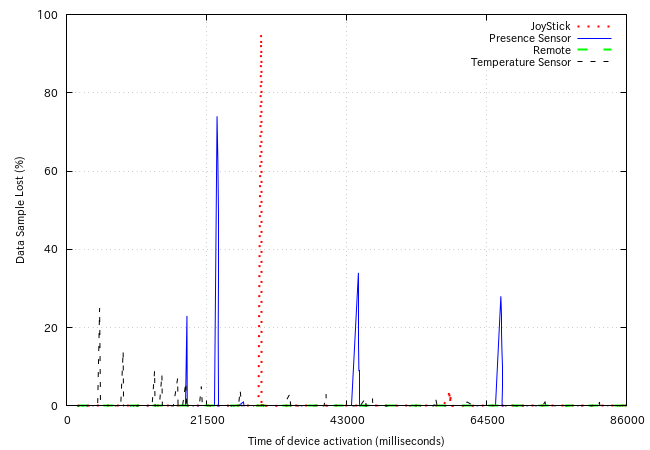
\includegraphics[width=1\linewidth]{transcient}
        \caption{Transient Time of Devices.}
        \label{fig:transcient}
    \end{figure}
\end{center}
The start times are that of the beginning of data production, which indicates the
powering on of the sensory devices.\\\\
APT-MAC gets better when it is run for a longer time. When the running time for an
APT-MAC device is maximized, the better the protocol gets. It can been seen from
figures \ref{fig:20-D-DLSR} and \ref{fig:20-D-DL}, TDMA protocol performs better in
the cases 3 and 4 of the short run for 20 devices \ref{tab:WSD}.\\\\
\newline
\begin{center}
    \begin{figure}[p]
        \begin{subfigure}{1\textwidth}
            \centering
            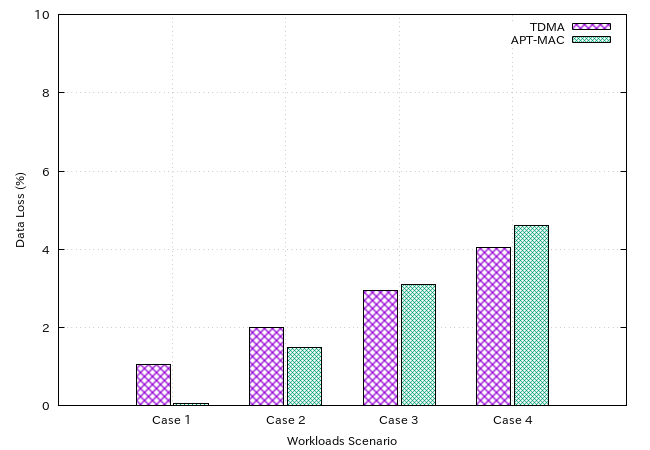
\includegraphics[width=0.8\linewidth]{20-1-data-loss-short-period}
            \caption{20 Devices : Data Loss Short Run.}
            \label{fig:20-D-DLSR}
        \end{subfigure}
        \begin{subfigure}{1\textwidth}
            \centering
            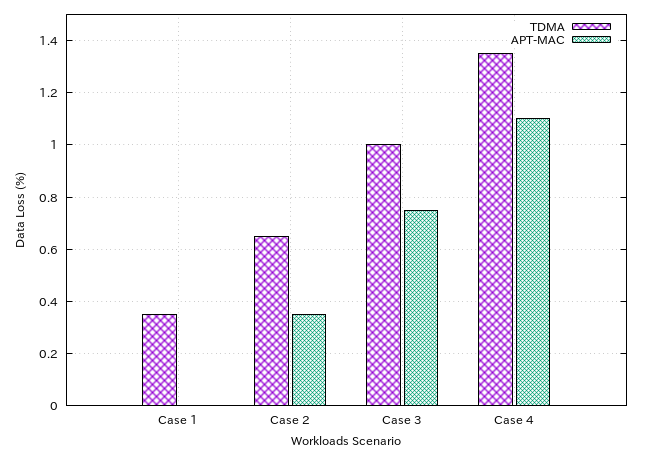
\includegraphics[width=0.8\linewidth]{20-1-data-loss}
            \caption{20 Devices : Data Loss}
            \label{fig:20-D-DL}
        \end{subfigure}
        \begin{subfigure}{1\textwidth}
            \centering
            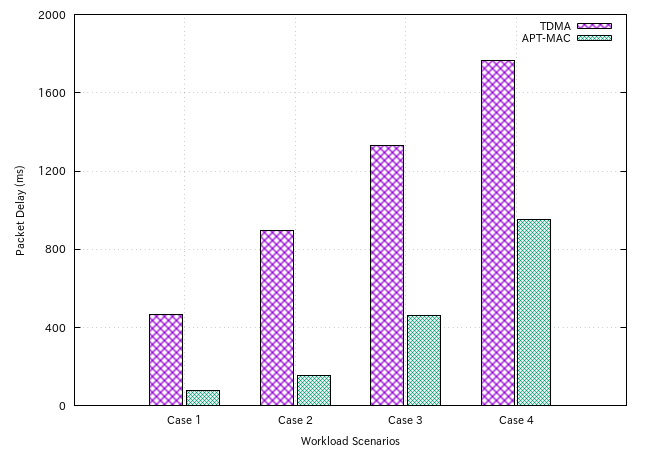
\includegraphics[width=0.8\linewidth]{20-1-packet-delay}
            \caption{20 Devices : Packet Delay}
            \label{fig:20-D-PD}
        \end{subfigure}
    \end{figure}
    \begin{figure}[p]
        \begin{subfigure}{1\textwidth}
            \centering
            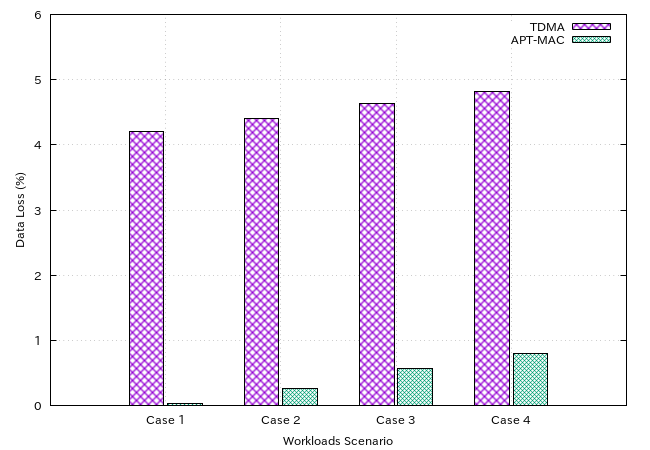
\includegraphics[width=1\linewidth]{30-data-loss}
            \caption{30 Devices : Data Loss}
            \label{fig:30-D-DL}
        \end{subfigure}
        \begin{subfigure}{1\textwidth}
            \centering
            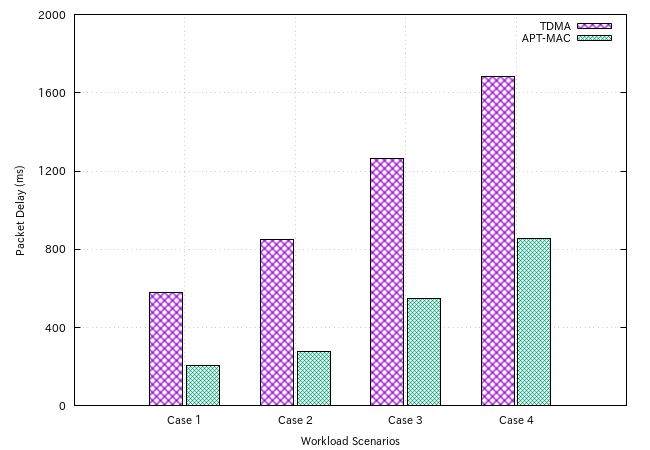
\includegraphics[width=1\linewidth]{30-packet-delay}
            \caption{30 Devices : Packet Delay}
            \label{fig:30-D-PD}
        \end{subfigure}
    \end{figure}
    \begin{figure}[p]
        \begin{subfigure}{1\textwidth}
            \centering
            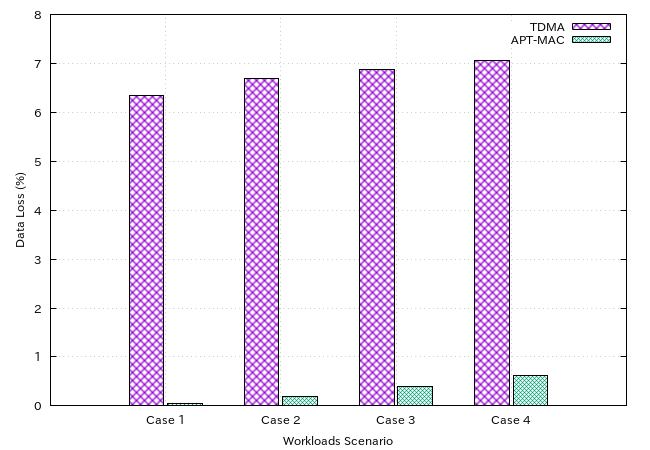
\includegraphics[width=1\linewidth]{40-data-loss}
            \caption{40 Devices : Data Loss}
            \label{fig:40-D-DL}
        \end{subfigure}
        \begin{subfigure}{1\textwidth}
            \centering
            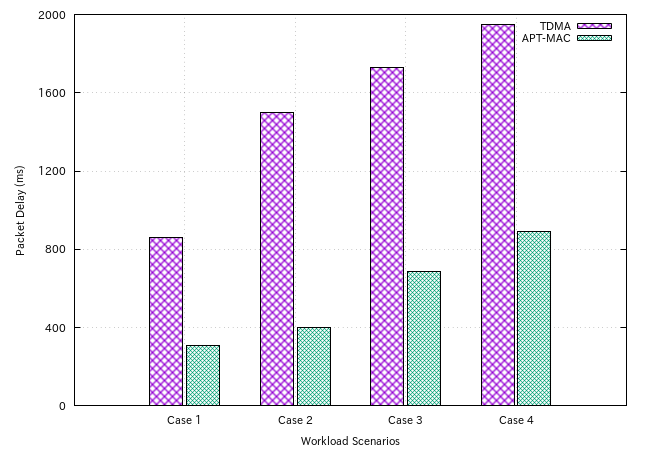
\includegraphics[width=1\linewidth]{40-packet-delay}
            \caption{40 Devices : Packet Delay}
            \label{fig:40-D-PD}
        \end{subfigure}
    \end{figure}
\end{center}
Packet delay, urgency to which packets are delivered to the reader in an equilibrium
state, for 20 devices of the various cases in table \ref{tab:WSD} is shown in figure
\ref{fig:20-D-PD}.
In both APT-MAC and TDMA, the time it takes to deliver new data
almost doubles from case 1 to case 2. It doubles for APT-MAC and almost plateaus for
TDMA in cases 3 to 4. Generally, APT-MAC delivers new data faster with a worse case
(case 4) time of $0.9$\textit{s} while that of TDMA is $1.7628$\textit{s}. On the
average, APT-MAC delivers new packet $2.7$ faster compared to TDMA - average of
$1.115$\textit{s} for TDMA and $0.411$\textit{s} for APT-MAC. Figure
\ref{fig:30-D-PD} and \ref{fig:40-D-PD} show packet delay for 30 and 40 devices 
respectively, similar trend is seen as that of 20 sensory devices with a gradual
increases as number of sensory devices increases.\\\\
Figure \ref{fig:20-D-DL} depicts the data loss, percentage of new data that is lost
as a result of untimely query, for 20 devices.
TDMA losses between $0.35\%$ in case 1 to $1.35\%$ in case 4 while APT-MAC does not
lose any new data in case 1 and the worse case, case 4, losses $1.10\%$. The data
loss doubles across the various cases for both protocols. The trend is similar as the
number devices increases - 30 \& 40 devices - figures \ref{fig:30-D-PD} and
\ref{fig:40-D-PD}, with the data loss of the APT-MAC being $0.8\%$ and $0.625\%$ for
30 \& 40 devices respectively. Proving that the more the sensory devices are the
better APT-MAC gets which is contrary to TDMA.


























 % Experimental Setup

\chapter{Conclusion}
Simulating a novel medium access control (MAC) protocol, APT-MAC - an adaptive
protocol to the data needs of the nodes accessing the medium, on the NS-3 platform
was the goal of this experiment. The aim was extended to investigate how the
performance of APT-MAC compare to that of TDMA.\\\\
The algorithm of the data-requirement-adaptive protocol is based on a solution to
the Multi-arm Bandit problem, more precisely $\varepsilon$-greedy algorithm, hence
the opening of this documentation sought to shed light on the Multi-arm Bandit
problem with its $\varepsilon$-greedy algorithm solution. A brief explanation of
TDMA was also introduced.
Next, was a description of the actual simulation, the various classes and the
task of the various functions used in the simulation. Three categories of 
tag-augmented data-packet producing sensory nodes were replicated, namely -
periodic, event-based and real-time. Both readers, that implementing TDMA and
APT-MAC respectively. The focus was turn on measuring the performance of both
TDMA and APT-MAC and an elucidation on how the variables of interest - data loss
and packet delay - were harnessed.\\\\
The results clearly showed that the performance outcome, that is, the percentage of
new data that is lost by the sensory devices and the speed, in terms of time, with
which a newly generated packet is delivered to reader due to the readers inability
or ability to query the tags on time is much better with APT-MAC.
In the worse case scenario, data loss and packet delay of APT-MAC were less than
$1\%$ and $0.9$\textit{s} respectively, and that of TDMA stood at $7.05\%$ for
data loss and almost $2$\textit{s} with TDMA.
\section{Future Work}
A follow up on this investigation could focus on the effects of mobility of the
tag-augmented sensory devices on the performance of the protocol. There are other
solutions to the Multi-Arm bandit problem, chief among them is the Upper Confidence
Bounds \cite{Sutton&Barto}. An investigation into which other algorithm could
perform better than $\varepsilon$-greedy algorithm is the focus of a future work
on this.


 % Experiment 1

%\input{Chapters/Chapter5} % Experiment 2

%\input{Chapters/Chapter6} % Results and Discussion

%\input{Chapters/Chapter7} % Conclusion

%% ----------------------------------------------------------------
% Now begin the Appendices, including them as separate files

\addtocontents{toc}{\vspace{2em}} % Add a gap in the Contents, for aesthetics

%\appendix % Cue to tell LaTeX that the following 'chapters' are Appendices

%\chapter{An Appendix}

Lorem ipsum dolor sit amet, consectetur adipiscing elit. Vivamus at pulvinar nisi. Phasellus hendrerit, diam placerat interdum iaculis, mauris justo cursus risus, in viverra purus eros at ligula. Ut metus justo, consequat a tristique posuere, laoreet nec nibh. Etiam et scelerisque mauris. Phasellus vel massa magna. Ut non neque id tortor pharetra bibendum vitae sit amet nisi. Duis nec quam quam, sed euismod justo. Pellentesque eu tellus vitae ante tempus malesuada. Nunc accumsan, quam in congue consequat, lectus lectus dapibus erat, id aliquet urna neque at massa. Nulla facilisi. Morbi ullamcorper eleifend posuere. Donec libero leo, faucibus nec bibendum at, mattis et urna. Proin consectetur, nunc ut imperdiet lobortis, magna neque tincidunt lectus, id iaculis nisi justo id nibh. Pellentesque vel sem in erat vulputate faucibus molestie ut lorem.

Quisque tristique urna in lorem laoreet at laoreet quam congue. Donec dolor turpis, blandit non imperdiet aliquet, blandit et felis. In lorem nisi, pretium sit amet vestibulum sed, tempus et sem. Proin non ante turpis. Nulla imperdiet fringilla convallis. Vivamus vel bibendum nisl. Pellentesque justo lectus, molestie vel luctus sed, lobortis in libero. Nulla facilisi. Aliquam erat volutpat. Suspendisse vitae nunc nunc. Sed aliquet est suscipit sapien rhoncus non adipiscing nibh consequat. Aliquam metus urna, faucibus eu vulputate non, luctus eu justo.

Donec urna leo, vulputate vitae porta eu, vehicula blandit libero. Phasellus eget massa et leo condimentum mollis. Nullam molestie, justo at pellentesque vulputate, sapien velit ornare diam, nec gravida lacus augue non diam. Integer mattis lacus id libero ultrices sit amet mollis neque molestie. Integer ut leo eget mi volutpat congue. Vivamus sodales, turpis id venenatis placerat, tellus purus adipiscing magna, eu aliquam nibh dolor id nibh. Pellentesque habitant morbi tristique senectus et netus et malesuada fames ac turpis egestas. Sed cursus convallis quam nec vehicula. Sed vulputate neque eget odio fringilla ac sodales urna feugiat.

Phasellus nisi quam, volutpat non ullamcorper eget, congue fringilla leo. Cras et erat et nibh placerat commodo id ornare est. Nulla facilisi. Aenean pulvinar scelerisque eros eget interdum. Nunc pulvinar magna ut felis varius in hendrerit dolor accumsan. Nunc pellentesque magna quis magna bibendum non laoreet erat tincidunt. Nulla facilisi.

Duis eget massa sem, gravida interdum ipsum. Nulla nunc nisl, hendrerit sit amet commodo vel, varius id tellus. Lorem ipsum dolor sit amet, consectetur adipiscing elit. Nunc ac dolor est. Suspendisse ultrices tincidunt metus eget accumsan. Nullam facilisis, justo vitae convallis sollicitudin, eros augue malesuada metus, nec sagittis diam nibh ut sapien. Duis blandit lectus vitae lorem aliquam nec euismod nisi volutpat. Vestibulum ornare dictum tortor, at faucibus justo tempor non. Nulla facilisi. Cras non massa nunc, eget euismod purus. Nunc metus ipsum, euismod a consectetur vel, hendrerit nec nunc.
	% Appendix Title

%\input{Appendices/AppendixB} % Appendix Title

%\input{Appendices/AppendixC} % Appendix Title

%\addtocontents{toc}{\vspace{2em}}  % Add a gap in the Contents, for aesthetics
\backmatter

%% ----------------------------------------------------------------
\label{Bibliography}
\lhead{\emph{Bibliography}}  % Change the left side page header to "Bibliography"
\bibliographystyle{unsrtnat}  % Use the "unsrtnat" BibTeX style for formatting the Bibliography
\bibliography{Bibliography}  % The references (bibliography) information are stored in the file named "Bibliography.bib"

\end{document}  % The End
%% ----------------------------------------------------------------
